% Copyright 2021 Thomas Ascher
% SPDX-License-Identifier: CC-BY-SA-4.0

\documentclass[a4paper,parskip=half]{scrartcl}

\usepackage[T1]{fontenc}
\usepackage[ngerman]{babel}
\usepackage{csquotes}
\usepackage[regular,condensed,sfdefault]{roboto}
\usepackage{graphicx}
\usepackage{chemformula}
\usepackage{amsmath,amsfonts,amssymb}
\usepackage[italic,symbolgreek]{mathastext}
\usepackage[backend=biber]{biblatex}
\usepackage[hidelinks,pdfencoding=auto,
  pdfauthor={Thomas Ascher},
  pdfusetitle,
  pdfkeywords={Bier,Kegging,Zapfanlage}]{hyperref}
\usepackage{microtype}

\addto\extrasngerman{
\def\figureautorefname{Abb.}
}

\addto\captionsngerman{
\renewcommand{\figurename}{Abb.}
}

\title{Alkoholmessung mit dem Refraktometer}
\author{Thomas Ascher}
\date{14. August 2021, \href{http://creativecommons.org/licenses/by-sa/4.0/}{CC BY-SA 4.0}}

\addbibresource{refraktometer.bib}

\newcommand{\bxi}{\mathit{B}_i}
\newcommand{\bxic}{\mathit{Bc}_i}
\newcommand{\bxf}{\mathit{B}_f}
\newcommand{\bxfc}{\mathit{Bc}_f}
\newcommand{\fg}{\mathit{FG}}
\newcommand{\abv}{\mathit{ABV}}
\newcommand{\abw}{\mathit{ABW}}


\begin{document}
\maketitle

\section*{Einleitung}

stabiler, schnellere Probenkühlung,
\autocite{Terrill2013}

nicht besser als Hydrometer
\autocite{Terrill2011}

\section*{Messprinzip eines Refraktometers}

The International Commission for Uniform Methods of Sugar Analysis  Ltd. (ICUMSA) -> Umrechnung.

Je dichter Flüssigkeit, desto langsamer licht durch,, Prisma misst, , dichter stärkere Brechung.  R = Verhältnis von licht im
Vakuum zu licht in der Flüssigkeit.
Kalibriert auf bestimmte Lösung bei bestimmter Temperatur,
Brix 20 °C
\autocite{Bonham2001}


maß wie licht abgebremst wird durch probe,
misst brechungsindex, optisches messen, licht durch probe, abgelenkt
prisma auf linse projiziert auf Fadennetz mit Skala, ansicht in Okular
Farblichen farbloser Bereich
auf verschiedene anwendungen kalibrierte skala, z.b. Brix.
1Bx = 1g Saccharose (Haushaltszucker) auf 99g Wasser. ähnlich zu plato
gleich behandelt
digital refraktometer -> licht intefferenz, verschiedene skalen, messbereich
ATC -> bimetall streifen, ATC nicht für Würze geeignet, falsche Korrektur
nicht für jede Substanz geeiget, ATC 10-30°C
\autocite{Terrill2013}

ATC verursacht fehler weil auf Zucker geeicht
\autocite{Terrill2010}

SG skala ungenau
\autocite{Terrill2011}

andere Temperatur verursacht verzerrung
ASBC refractometry protocols, Kurfenanpassung pro würze
\autocite{Bonham2001}

ATC nicht
für alle Probe geeignet. -> sugar Water
\autocite{Depalma2017}

Refi misst index Lichtbrechung
mehr alk -> höhere RI
Dichte Temperatur abhängig, 20°C
\autocite{Gossett2012}

analog refractometer performed as well as the bench-top, digital refractometer
problems develop that limit precision.  For example, some dark and turbid samples will give rather fuzzy lines of demarcation when one tries to read the analog scale.  Often this fuzziness gets worse with time as the sample sits on the glass slide, presumably as solids settle or gas bubbles form.  The fuzziness of the demarcation line serves as a kind of warning to the user. 
mehrfache Messung bei digitalen
\autocite{Gossett2012a}

\section*{Hydrometer}

Auftrieb, = gewicht der verdrängten flüssigkeit, sinkt weiter
ein bei weniger dichten Würze.
100 bis 200 ml Probe
co2 in Lösung beeinflusst den Messwert um circa 0.3 P
Refraktometer weniger einfluss durch co2
Messung fg zu niedrig wegen Alkoholfehler
\autocite{Novotny2017}

\autocite{Kunze2004}

\autocite{Brueckelmeier2018}

\autocite{Narziss2009}

\section*{Kalibrierung und Justierung}

2 punkt 20°C, 0 Stellung jeden Tag, Wasser 0° Bx, Referenzlösung herstellen,
mit kalibrierter Feinwaage
\autocite{Terrill2013}

Kalibrierung bei Umgebungstemperatur.
\autocite{Bonham2001}

Deionisiertes Wasser und Kalibrierung auf 0, NIST standard
organisation
\autocite{Depalma2017}

Rene Fehler von 2 Brix.

\section*{Würze-Korrekturfaktor}

WCF = refrakto / hydro, 1.02-1.06, 1.04 guter Durchschnitt. Abhängig von Würze
Mehr adjunkte kleinerer Faktor
\autocite{Terrill2013}

Dichte Lösung Zucker nicht dichte Würze
RI 15 \% Maltose 1,3362, Succrose 1,3557 15.3, 
WCF = refrakto Bx  / Hydro in P
\autocite{Bonham2001}

\section*{Messung durchführen}

einige Tropfen auf Refi, nicht heiß tropfen lassen, verschlossen auskühlen
\autocite{Terrill2013}

trocken und sauber
\autocite{Bonham2001}

Möglichst genau durchführen, 0.25 P in Hydrometer Fehler,
0.25 \% ABV Fehler
\autocite{Bonham2001}

Messfehler durch fehlende Temperaturkontrolle, ATC nicht
für alle Probe geeignet.
Kreuzkontaminierung durch schlecht gereinigte
\autocite{Depalma2017}


\section*{Korrelationsfunktionen zur Schätzung des scheinbaren Restextrakts}

durch alkoholfehler misst nicht AE, dnerer RI, Korrelation notwendig.
\autocite{Terrill2010a}

linearer zusammenhang zwischen Vergärungsgrad und Alkoholgehalt,
gleicher RI für verschiedene Probenzusammensetzung.
\autocite{Terrill2010}

Temperatur abhängig, 20°C
\autocite{Gossett2012}

\subsection*{Gardner (2000)}

% equations derived by Roberts & Stewart: 1
ausreichend genau für den Heimbereich
\autocite{Bonham2001}

\begin{equation}
\mathit{AE}=1.53 \cdot \bxf - 0.59 \cdot \bxic
\label{eq:gardner} 
\end{equation}

\begin{equation}
\abw = 1.09 \cdot \bxf - 1.13 \cdot \mathit{AE}
\end{equation}


\subsection*{Bonham (2001)}

Standard \autocite{Terrill2010a}

Laut Gossett Bonham formel falsch angewendet Bx korrigiert.
Gemessen 10 Biere bei Stammwürze von 9 - 24 und bei Standard Formel Abweichungen
beim AE festgestellt von 0.1 - 2.2 Plato, keine Abweichung bei
58\% RDF (71\% ADF), mean = 1.3 °Plato
\autocite{Terrill2010a}

Quelle nicht bekannt, auch wenn korrekt insignifikante verbesserung
\autocite{Terrill2011}

\autocite{Bonham2001}

\begin{align}
\begin{split}
\fg &= 1.001843 - 0.002318474 \cdot \bxic - 0.000007775 \cdot \bxic^2 -
0.000000034 \cdot \bxic^3 \\
& \quad + 0.00574 \cdot \bxf +
0.00003344 \cdot \bxf^2 + 0.000000086 \cdot \bxf^3
\end{split} \label{eq:bonham} 
\end{align}

\begin{align}
\begin{split}
\abv = \frac{(277.8851 - 277.4 \cdot \fg + 0.9956 \cdot \bxf + 0.00523 \cdot \bxf^2 + 0.000015 \cdot \bxf^3) \cdot \fg}{0.79}
\end{split}
\end{align}

\subsection*{Terrill (2011)}

12 Biere, 8 kommzerielle Brauereien evaluiert, 88 \% des AE liegt innerhalb
von 0.5 °P
\autocite{Terrill2013}

OE: 9 - 24, AE: 1.8 - 5.6, ADF - 73 \% to 91 \%, 60 Messungen,
\autocite{Terrill2010}


Bonham Formel quelle nicht bekannt
50 \% RDF (61 \% ADF) Proben gemessen wurden aber verworfen, weil
Genauigkeit verschlechtert.
Abweichungen bein linearen besser als vereinfachte Kubische
ADFs from 73 \% to 91 \% Ergebnisse
\autocite{Terrill2011}

mean, std, max, <0.5°P
old: -0.4, 0.6, -2.1, 41 \%
new cubic: 0.2, 0.3, 1.2, 85 \%
new linear 0.03, 0.4, 1.0, 84 \%

\autocite{Terrill2011}


\begin{equation}
\fg = 1 - 0.00085683 \cdot \bxic + 0.0034941 \cdot \bxfc
\label{eq:terrilllinear} 
\end{equation}

\begin{align}
\begin{split}
\fg &= 1 - 0.0044993 \cdot \bxic + 0.011774 \cdot \bxfc + 0.00027581 \cdot \bxic^2 - 0.0012717 \cdot \bxfc^2 \\
& \quad  - 0.0000072800 \cdot \bxic^3  + 0.000063293 \cdot \bxfc^3
\end{split} \label{eq:terrillcubic} 
\end{align}

\subsection*{Gossett (2012)}

unzufrieden mit indirekter Messwert mit Umrechnung von
unbekannter Genauigkeit.
Auswirkung von Alkoholgehalt auf den Brix Messung.
Stochiometrisches Modell. 12 Biere im Vergleich mit
Hydrometer. Kochen Verdünnung.
\autocite{Gossett2012}

0.445 Brix (20°C) per \% ABW, 
Standardabweichung bei 0.1 Brix Genauigkeit  \%ABV of 0.115/0.353 = 0.33
und Ausschluss systematischer Messfehler.
\autocite{Gossett2012a}

Formeln
\autocite{Gossett2012b}

\begin{equation}
k = 0.445
\end{equation}

\begin{equation}
C = 100 \cdot \frac{\bxi - \bxf}{100 - 48.4 \cdot k - 0.582 \cdot \bxf}
\end{equation}

\begin{equation}
\abw = \frac{48.4 \cdot C}{100 - 0.582 \cdot C}
\label{eq:gossett} 
\end{equation}

Bonham zur FG Bestimmung.

12 Biere Mittlere Abweichung 0.1 ABV, Standardabweichung 0.4 ABV
model std dev 0.2 \%ABV. beo 0.1 brix auflösung

\autocite{Gossett2012c}

\subsection*{Novotný (2017)}

Verglichen mit Terrill Formel 65-80 \% Vergärungsgrad genau,

Petr Kosin

3 Biere bei 11,6, 17, 22,9 OE, genauigkeit innerhlb von
0.26 °P, bei Hydrometer 0.15 °P abezogen wegen CO2
2 Tage besseres ergebnis als Terrill
\autocite{Novotny2017}

Vergleichwerte
\autocite{Novotny2017a}


\begin{equation} 
\fg = -0.002349 \cdot \bxic + 0.006276 \cdot \bxfc + 1
\label{eq:novotnylinear} 
\end{equation}

\begin{align}
\begin{split}
\fg &= 1.335 \cdot 10^{-5} \cdot \bxic^2 - 3.239 \cdot 10^{-5} \cdot \bxic \cdot \bxfc + 2.916 \cdot 10^{-5} \cdot \bxfc^2 \\
& \quad - 2.421 \cdot 10^{-3} \cdot \bxic + 6.219 \cdot 10^{-3} \cdot \bxfc + 1
\end{split} \label{eq:novotnyquadratic} 
\end{align}

\begin{equation} 
\abw = 0.67062 \cdot \bxic - 0.66091 \cdot \bxfc
\end{equation}

\begin{equation} 
\mathit{RE} = -0.29388 \cdot \bxic + 1.27582 \cdot \bxfc
\end{equation} 

\autoref{eq:novotnylinear}

%(\autoref{fig:groteblohm}) von 
%Grote \& Bohm \autocite{GroteBlohm2020}.

%\begin{figure}[h]
%\centering
%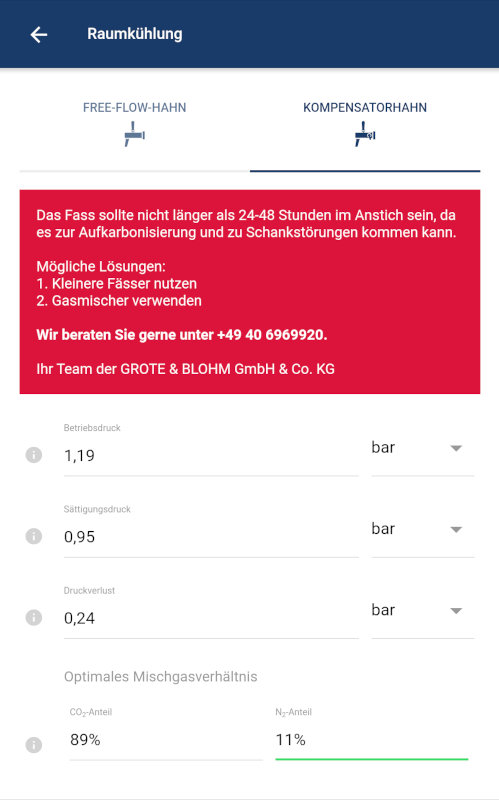
\includegraphics[width=4.8cm]{images/groteblohm.jpg}
%\caption{FOBB-APP}
%\label{fig:groteblohm}
%\end{figure}


\printbibliography[title=Quellen]

\end{document}